% This is samplepaper.tex, a sample chapter demonstrating the
% LLNCS macro package for Springer Computer Science proceedings;
% Version 2.20 of 2017/10/04
%
\documentclass[runningheads]{llncs}
%
\usepackage{graphicx}
\usepackage{amsmath}
% Used for displaying a sample figure. If possible, figure files should
% be included in EPS format.
%
% If you use the hyperref package, please uncomment the following line
% to display URLs in blue roman font according to Springer's eBook style:
% \renewcommand\UrlFont{\color{blue}\rmfamily}

\begin{document}
%
\title{Contribution Title}
%
%\titlerunning{Abbreviated paper title}
% If the paper title is too long for the running head, you can set
% an abbreviated paper title here
%
\author{First Author\inst{1}\orcidID{0000-1111-2222-3333} \and
Second Author\inst{2,3}\orcidID{1111-2222-3333-4444} \and
Third Author\inst{3}\orcidID{2222--3333-4444-5555}}
%
\authorrunning{F. Author et al.}
% First names are abbreviated in the running head.
% If there are more than two authors, 'et al.' is used.
%
\institute{Princeton University, Princeton NJ 08544, USA \and
Springer Heidelberg, Tiergartenstr. 17, 69121 Heidelberg, Germany
\email{lncs@springer.com}\\
\url{http://www.springer.com/gp/computer-science/lncs} \and
ABC Institute, Rupert-Karls-University Heidelberg, Heidelberg, Germany\\
\email{\{abc,lncs\}@uni-heidelberg.de}}
%
\maketitle              % typeset the header of the contribution
%
\begin{abstract}
The abstract should briefly summarize the contents of the paper in
150--250 words.

\keywords{First keyword  \and Second keyword \and Another keyword.}
\end{abstract}
%
%
%
\section{Introduction}
% \subsection{A Subsection Sample}
Classification is the problem of identifying to which a set if categories or sub-populations a new observation belongs, on the basis of a training set of data containing observations or instance whose category membership is known. In many domain, especially for big data and image recognition, classification has become a most hot and significant topic of research[1].In a training set, the information and features of a datum can be formally and numerically represented as a vector (x1,x2,...,xn). In such a n-dimensional features space, the main goal of classification is to estimate the label of a new unlabeled vector from a testing dataset through calculating the similarity among the labeled and unlabeled vectors. Generally, there is a common hypothesis that the training dataset and the testing dataset has a semblable distribution. 

As a well known and widely used method, the k nearest neighbor (KNN) method, looked on as the most simple but effective method among many available classification method such as bayesian method, support vector machine and neural network. Due to its simplicity but good performance, the kNN algorithm has been considered as a top-10 data-mining method[2]. Known as a supervised learning algorithm, its working mechanism is fairly easy to grasp: for a given test sample, KNN algorithm try to get the nearest k samples in the training data set based on a specific distance metric, and then predict according to the information of these samples. In a classification problem, the vote method is usually applied to predict the class of one test samples. i.e. label this sample the most common class among the k nearest neighbors. In the past few decades, some researches are also carried on to replace the vote method with other case based reasoning method, for instance, [3][4] used evidence KNN based on the Dempster-Shafer Theory to extend the classical vote method.

Also, there are two issues often come into being discussed in the research: The First is about the similarity and distance compute between different vectors. recently many new algorithm has been proposed to solve this issue, Lin et al. [5] proposed a similarity compute method via fusing neighborhood information. In this proposed algorithm, both the euclidean distance and the neighbor information is considered simultaneously, the two metric is combined together to measure the similarity between samples. Yung-Kyun Noh et al.[6] proposed a generative metric learning method to enhance the performance of kNN algorithm. The second issue is about the selection of optimal value of k for a given data set. The general kNN algorithm simply  assume the whole data set share a same value of k, which is actually not proper and inaccurate for a finite and non-uniformly distributed data set.Recently, many new method has been generate to find the k value adaptively or determine a k value for different sample respectively,  Nicolás García-Pedrajas et al. [7] propose a algorithm to obtain local k value with a simple and fast procdeure, Zhang et al. [8] propose to learn a correlation matrix to reconstruct test data points by training data to assign different k values to different test data points.

The drawbacks of the foregoing methods is obvious, they ignore the uncertainty the training data sample itself. As we all know, the training dataset is composed of a group of labeled data samples, the label itself usually decided by some experts however, could be imprecise or even incorrect.While the label information of the k neighbors is combined to make the ultimate decision, the uncertainty of each point also accumulate. In this case, the accuracy of the kNN algorithm will decrease to some extent. Fortunately, a lot of additional and available information can used to quantify the uncertainty of the label of the sample itself. In a recommendation system, a rate of users or votes of experts of a history result could be considerated when quantify the uncertainties. For instance, Zhu et al.[9] described a a real-world decision support system for multi-disciplinary treatment called MdtDSS, the core recommend system predict a new patient's therapeutic regimen based on the historic patients. The ultimate therapy of one patient is voted by a group of doctor which reflect the doctors' opinion. The vote result of one doctor express if he/she approve the ultimate therapy of this person. Obviously, we can construct some connection between the vote result and the uncertainties.

In this paper, we define a method to quantify the uncertainties of samples in the training dataset with extra information, later, we fuse both the uncertainty and the label information as the evidence of that sample in the k nearest neighbors. Then, as to combine all these evidences, we use Dempster-shafer theory to accumulate  all these evidences to decide which class a test sample belongs to. Later, we proposed two strategy to select the optimal k value for a specific test sample based on the combined evidences. At last, we carry on a series of experiments with the data in the MdtDSS mentioned in [9] to verify our method.

This paper is organized as follows: In section 2, we discuss related work on kNN algorithms. In section 3, we introduce the Dempster-shafer evidence theory and the MdtDSS. In section 4, we present the modified evidence-theory based on the uncertainty of data sample and the 2 algorithms upon optimal k value selection for this sample. Finally, in the section 5, we carry on several experiments and present results.


\section{Related Work}
Although the majority vote rule make the kNN algorithm more simple and easier to carry, it is based on a assumption that each of the K nearest neighbors is equally important. In practice, the circumstances can be more complex.Intuitively, the closer the neighbor, the more possible that the unknown vector f will be in the class of this neighbor. In 1995, Thierry Denœux[3] unprecedentedly define the frame of discernment [10] of a kNN method, and used  the distance of samples to measure the mass function of one sample. Our own work is a extend to his work.

To replace the majority vote rule, some researchers are also prone to looking on the relationship between the global  and local probability distribution. For a small training data, Sunsern Cheamanunkul [11] propose a simple k-NN rule that takes into account the labels of all of the neighbors, rather than just the most common label. In his approach, relative entropy is used to measure the relationship between the global  and local probability distribution.

\section{Preliminary}
\subsection{Dempster-Shafer theory}
As a generalization of the Bayesian theory of subjective probability, Dempster Shafer theory was proposed in 1976 in [10]. It is a general framework for reasoning with uncertainty data. This theory provide a model to express know and unknown directly of different sources, and the ability to combine all the evidence. It mainly contains 2 crucial steps: Basic Belief Assignment(BBA) and evidence combination.

In the first step, let U represent a non-empty set of mutually exclusive and exhaustive propositions called the frame of decrement. The power set $2^{U}$ is all subsets of the set U, which includes both the empty set  and the entire set U. For the frame of discernment U, the function m:$2^{u}$ $\rightarrow$ [0,1] is a basic probability assignment (BPA) also called a mass function. This function satisfies the following two conditions:

\begin{equation}
\begin{split}
&(1)\ m(\phi) = 0\\&(2)\ \sum_{A\subset U}m(A) = 1
\end{split}
\end{equation}

m(A) indicates the degree of trust exactly in A. The subsets A of U where m(A) > 0 are called the focal elements of the belief function, and their union is called its core. The function Bel:$2^{u}$ $\rightarrow$ [0,1] is the belief function over U, is defined as the sum of all the masses of subsets:

\begin{equation}
Bel(A) = \sum_{B\subset A}m(B)
\end{equation}

Belief (usually denoted Bel) measures the strength of the evidence in favor of a proposition but not any of its subsets. It ranges from 0 (indicating no evidence) to 1 (denoting certainty). An important difference with probability theory is the sum of belief of a proposition and its negation not necessarily equal to 1. Hence, the remaining belief of A, called total ignorance, is the belief of the whole frame of discernment.

In the second step, Dempster Shafer define a method to combine two or more mass assignments of a same frame of discernment in specific situations. To combine there assignments means to accumulate all evidence from all sources in one frame.This rule derives common shared beliefs among multiple sources and ignores all the conflicting (non-shared) beliefs through a normalization factor. 

Given n mass functions $m_1$,$m_2$...$m_n$ on the same frame of discernment U, for arbitrary A  included in U, the combination rule is as follow:


\begin{equation}
\begin{split}
&\ m_{1,2,...,n}(\phi) = 0\\
&\ 
\begin{split}
m_{1,2,...,n}(A)  &\ =(m_1\oplus m_2 \oplus \cdots 
\oplus m_n)(A) \\
&\ = \frac{1}{K} \sum_{A_1 \cap A_2 \cap \cdots
\cap A_n} m_1(A_1) \cdot m_2(A_2) \cdots m_n(A_n)
\end{split}
\end{split}
\end{equation}

where:

\begin{equation}
\begin{split}
K &\ = \sum_{A_1 \cap A_2 \cap \cdots
\cap A_n \ne \phi} m_1(A_1) \cdot m_2(A_2) \cdots m_n(A_n) \\
&\ = 1 - \sum_{A_1 \cap A_2 \cap \cdots
\cap A_n = \phi} m_1(A_1) \cdot m_2(A_2) \cdots m_n(A_n) 
\end{split}
\end{equation}

the K called Normalization factor is a measure of the amount of conflict among mass functions. 


\subsubsection{Sample Heading (Third Level)} Only two levels of
headings should be numbered. Lower level headings remain unnumbered;
they are formatted as run-in headings.

\paragraph{Sample Heading (Fourth Level)}
The contribution should contain no more than four levels of
headings. Table~\ref{tab1} gives a summary of all heading levels.

\begin{table}
\caption{Table captions should be placed above the
tables.}\label{tab1}
\begin{tabular}{|l|l|l|}
\hline
Heading level &  Example & Font size and style\\
\hline
Title (centered) &  {\Large\bfseries Lecture Notes} & 14 point, bold\\
1st-level heading &  {\large\bfseries 1 Introduction} & 12 point, bold\\
2nd-level heading & {\bfseries 2.1 Printing Area} & 10 point, bold\\
3rd-level heading & {\bfseries Run-in Heading in Bold.} Text follows & 10 point, bold\\
4th-level heading & {\itshape Lowest Level Heading.} Text follows & 10 point, italic\\
\hline
\end{tabular}
\end{table}


\noindent Displayed equations are centered and set on a separate
line.
\begin{equation}
x + y = z
\end{equation}
Please try to avoid rasterized images for line-art diagrams and
schemas. Whenever possible, use vector graphics instead (see
Fig.~\ref{fig1}).

\begin{figure}
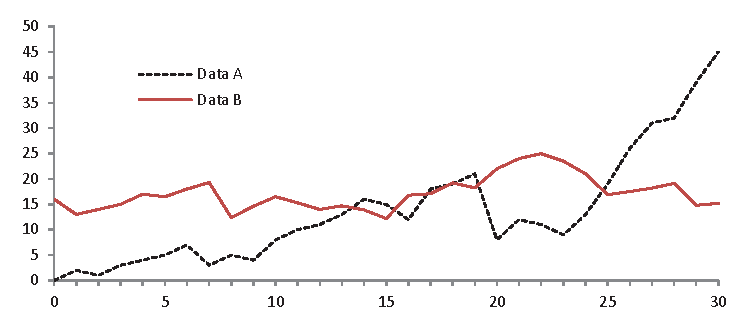
\includegraphics[width=\textwidth]{fig1.eps}
\caption{A figure caption is always placed below the illustration.
Please note that short captions are centered, while long ones are
justified by the macro package automatically.} \label{fig1}
\end{figure}

\begin{theorem}
This is a sample theorem. The run-in heading is set in bold, while
the following text appears in italics. Definitions, lemmas,
propositions, and corollaries are styled the same way.
\end{theorem}
%
% the environments 'definition', 'lemma', 'proposition', 'corollary',
% 'remark', and 'example' are defined in the LLNCS documentclass as well.
%
\begin{proof}
Proofs, examples, and remarks have the initial word in italics,
while the following text appears in normal font.
\end{proof}
For citations of references, we prefer the use of square brackets
and consecutive numbers. Citations using labels or the author/year
convention are also acceptable. The following bibliography provides
a sample reference list with entries for journal
articles~\cite{ref_article1}, an LNCS chapter~\cite{ref_lncs1}, a
book~\cite{ref_book1}, proceedings without editors~\cite{ref_proc1},
and a homepage~\cite{ref_url1}. Multiple citations are grouped
\cite{ref_article1,ref_lncs1,ref_book1},
\cite{ref_article1,ref_book1,ref_proc1,ref_url1}.
%
% ---- Bibliography ----
%
% BibTeX users should specify bibliography style 'splncs04'.
% References will then be sorted and formatted in the correct style.
%
% \bibliographystyle{splncs04}
% \bibliography{mybibliography}
%
\begin{thebibliography}{8}
\bibitem{ref_article1}
Author, F.: Article title. Journal \textbf{2}(5), 99--110 (2016)

\bibitem{ref_lncs1}
Author, F., Author, S.: Title of a proceedings paper. In: Editor,
F., Editor, S. (eds.) CONFERENCE 2016, LNCS, vol. 9999, pp. 1--13.
Springer, Heidelberg (2016). \doi{10.10007/1234567890}

\bibitem{ref_book1}
Author, F., Author, S., Author, T.: Book title. 2nd edn. Publisher,
Location (1999)

\bibitem{ref_proc1}
Author, A.-B.: Contribution title. In: 9th International Proceedings
on Proceedings, pp. 1--2. Publisher, Location (2010)

\bibitem{ref_url1}
LNCS Homepage, \url{http://www.springer.com/lncs}. Last accessed 4
Oct 2017
\end{thebibliography}
\end{document}
